\section{Results}
\label{sec:results}

All three pre-registered conditions hold, so H1 is accepted. \hh{} is not worse than Hydra
and not worse than the symmetric control in accuracy, and its transform is $11.2\times$
faster than Hydra's. The accuracy result is one of equivalence, not superiority, and it is
not shown on the UEA datasets alone. All tables in this section are generated from the
stored results (Section~\ref{sec:reproducibility}).

\subsection{Primary endpoint}

\begin{table}[t]
\centering\small
% Generated by experiments/paper_tables.py; do not edit by hand.
\begin{tabular}{lrrlcc}
\toprule
Comparison & Means (\%) & $\Delta$ & W/T/L & $P$(left / rope / right) & $P$(not worse) \\
\midrule
vs Hydra & 84.37 vs 84.43 & $-0.06$ & 47/5/86 & 0.012 / 0.988 / 0.000 & \textbf{0.988} \\
vs \texttt{control\_sym} & 84.37 vs 84.33 & $+0.04$ & 64/7/67 & 0.000 / 1.000 / 0.000 & \textbf{1.000} \\
vs \texttt{control} & 84.37 vs 84.26 & $+0.11$ & 72/5/61 & 0.000 / 1.000 / 0.000 & \textbf{1.000} \\
\bottomrule
\end{tabular}

\caption{Primary endpoint: \hh{} against each arm over 138 datasets (dataset means over 30
resamples, percentage points). $\Delta$ is \hh{} minus the comparator; W/T/L counts
datasets. Bayesian signed-rank test with ROPE $\pm0.5$; bold: $P(\text{not worse})\ge
0.95$.}
\label{tab:primary}
\end{table}

\begin{table}[t]
\centering\small
% Generated by experiments/paper_tables.py; do not edit by hand.
\begin{tabular}{lr}
\toprule
Quantity (median over datasets) & Value \\
\midrule
Hydra / Hanner-Hydra transform time & 11.23$\times$ \\
\texttt{control\_sym} / Hanner-Hydra & 3.79$\times$ \\
Hydra / \texttt{control\_sym} & 2.99$\times$ \\
Smallest Hydra / Hanner-Hydra ratio & 4.06$\times$ \\
Datasets & 138 \\
\bottomrule
\end{tabular}

\caption{Single-core transform time (Apple M4, one thread). Per dataset, the median of
three pass medians; the table gives the median over datasets of the per-dataset ratios.}
\label{tab:timing}
\end{table}

Table~\ref{tab:primary} gives the accuracy comparisons. Against Hydra, the mean accuracy is
84.37\% against 84.43\% ($\Delta=-0.06$ points), and the posterior probability that \hh{}
is not worse is 0.988, all of it from the ROPE. Against \texttt{control\_sym} and
\texttt{control}, the posterior lies entirely in the ROPE. The differences per dataset are
small but not uniform. \hh{} loses more datasets to Hydra than it wins (47/5/86), with a
median difference of $-0.10$ points. On 18 of the 138 datasets the difference exceeds 2
points in either direction, from $-5.43$ (FreezerSmallTrain) to $+6.79$
(SemgHandMovementCh2).

Table~\ref{tab:timing} gives the timing endpoint. The median ratio of Hydra's transform time
to \hh{}'s is $11.23\times$, with a bootstrap 95\% interval of 10.23--12.01; the medians
of the three passes are $11.17\times$, $11.24\times$ and $11.24\times$. Every dataset is
above the pre-registered threshold of $4\times$. The ratio is $11.76\times$ on the UCR
datasets and $9.38\times$ on the UEA datasets. Summed over all datasets, one transform of
every test set takes 29.0 minutes with Hydra and 2.2 minutes with \hh{}.

\subsection{Where the speed comes from}

The controls split the speed-up into two parts. \texttt{control\_sym} runs in a Numba
kernel like \hh{}'s, but evaluates every vertex of its groups as a dense ternary dot
product instead of following a cotree. It is $2.99\times$ faster than Hydra and $3.79\times$
slower than \hh{}. The $3.79\times$ is the gain of the recursion over a dense ternary
evaluation of groups of the same size and sparsity. A ternary kernel that visits only the
non-zeros would need fewer operations (Table~\ref{tab:operations}), and we did not time
one, so $3.79\times$ is an upper bound on what the cotree adds over the best ternary
implementation (Section~\ref{sec:operations}). The operation counts are not a model of
these times: Hydra and the dense control have nearly the same count, but Hydra is
$2.99\times$ slower.

The ratio to Hydra is lowest on the two datasets with the most channels, DuckDuckGeese
($C=1{,}345$, $4.06\times$) and PEMS-SF ($C=963$, $4.83\times$), and on the dataset with
the longest series, StandWalkJump ($T=2{,}500$, $5.86\times$). It is highest for StarLightCurves
($23.15\times$). Seventeen datasets are below $8\times$.

\begin{table}[t]
\centering\small
% Generated by experiments/paper_tables.py; do not edit by hand.
\begin{tabular}{lr}
\toprule
Arm & Median extra peak memory (MB) \\
\midrule
Hanner-Hydra & 19 \\
\texttt{control} & 17 \\
\texttt{control\_sym} & 17 \\
Hydra & 450 \\
\midrule
Hydra / Hanner-Hydra (median of per-dataset ratios) & 23.8$\times$ \\
\bottomrule
\end{tabular}

\caption{Extra peak memory of the transform: the rise in peak resident set size during
\texttt{transform} of the test set, after \texttt{fit} and a warm-up, each measured in a
fresh process. It includes the output array.}
\label{tab:memory}
\end{table}

Memory follows the same pattern (Table~\ref{tab:memory}). The median extra peak of the
transform is 450\,MB for Hydra and 19\,MB for \hh{}, and the median of the per-dataset
ratios is $23.8\times$. Hydra needs more memory on all 138 datasets; the closest cases are
again DuckDuckGeese ($1.17\times$) and PEMS-SF ($1.32\times$). Its largest extra peak
is 16.8\,GB (StarLightCurves), against 421\,MB for \hh{} (Crop). The peak of \hh{} is
essentially its output: a median of 14\,MB of features and about 1\,MB of working memory,
the same as the controls. Fitting the transform, which samples the groups, takes a median
of 5\,ms for \hh{}, 1\,ms for Hydra and 28 and 38\,ms for the two controls, which draw
their vectors one at a time. All are negligible next to the transform.

\subsection{Subsets and secondary metrics}

\begin{table}[t]
\centering\small
% Generated by experiments/paper_tables.py; do not edit by hand.
\begin{tabular}{lrrrrr}
\toprule
Subset & Datasets & $\Delta$ vs Hydra & $P$(not worse) & $\Delta$ vs \texttt{control\_sym} & $P$(not worse) \\
\midrule
All & 138 & $-0.06$ & 0.988 & $+0.04$ & 1.000 \\
UCR & 112 & $+0.06$ & 0.999 & $+0.00$ & 1.000 \\
UEA & 26 & $-0.54$ & 0.220 & $+0.23$ & 1.000 \\
Fresh & 93 & $+0.01$ & 1.000 & $+0.04$ & 1.000 \\
\bottomrule
\end{tabular}

\caption{Pre-registered subsets. Fresh: the 93 datasets that informed no design choice.
$P$: posterior probability that \hh{} is not worse.}
\label{tab:subsets}
\end{table}

\begin{table}[t]
\centering\small
% Generated by experiments/paper_tables.py; do not edit by hand.
\begin{tabular}{llrrrr}
\toprule
Metric & Datasets & $\Delta$ vs Hydra & $P$(not worse) & $\Delta$ vs \texttt{control\_sym} & $P$(not worse) \\
\midrule
Accuracy & All (138) & $-0.06$ & \textbf{0.988} & $+0.04$ & \textbf{1.000} \\
Balanced accuracy & All (138) & $-0.16$ & 0.853 & $+0.03$ & \textbf{1.000} \\
Macro-F1 & All (138) & $-0.16$ & 0.788 & $+0.03$ & \textbf{1.000} \\
\midrule
Accuracy & UEA (26) & $-0.54$ & 0.220 & $+0.23$ & \textbf{1.000} \\
Balanced accuracy & UEA (26) & $-0.69$ & 0.133 & $+0.23$ & \textbf{1.000} \\
Macro-F1 & UEA (26) & $-0.76$ & 0.145 & $+0.20$ & \textbf{1.000} \\
\bottomrule
\end{tabular}

\caption{Accuracy, balanced accuracy and macro-F1, each analysed like the primary endpoint
(Bayesian signed-rank test, ROPE $\pm0.5$ points); bold: $P(\text{not worse})\ge0.95$.}
\label{tab:metrics}
\end{table}

Table~\ref{tab:subsets} repeats the analysis on the pre-registered subsets. On the 112 UCR
datasets, \hh{} is practically equivalent to Hydra ($+0.06$ points). On the 93 fresh
datasets the result is the same as on all datasets ($+0.01$), so it is not carried by the
datasets that informed the design. On the 26 UEA datasets, \hh{} is 0.54 points behind
Hydra, and \emph{not worse} cannot be shown ($P=0.22$). The gap is shared by the
ternary control, so it is not specific to the cotree: \texttt{control\_sym} is 0.77 points
behind Hydra on UEA, and
\hh{} is practically equivalent to both controls on every subset. The gap is largest on
the datasets with many channels, which Section~\ref{sec:discussion} discusses.

Balanced accuracy and macro-F1 show the same picture with a slightly larger gap
(Table~\ref{tab:metrics}). Against Hydra, \hh{} is 0.16 points behind on both over all
datasets, and \emph{not worse} is not shown ($P=0.853$ and $0.788$). The larger gap
suggests slightly larger losses on minority classes than on accuracy. Against \texttt{control\_sym}, it is
practically equivalent on every metric and subset.

\begin{table}[t]
\centering\small
% Generated by experiments/paper_tables.py; do not edit by hand.
\begin{tabular}{llrlrr}
\toprule
Pair & & $\Delta$ & W/T/L & $p$ & $p$ (Holm) \\
\midrule
Hanner-Hydra & vs \texttt{control\_sym} & $+0.04$ & 64/7/67 & 0.919 & 0.919 \\
Hanner-Hydra & vs \texttt{control} & $+0.11$ & 72/5/61 & 0.248 & 0.497 \\
Hanner-Hydra & vs Hydra & $-0.06$ & 47/5/86 & 0.054 & 0.216 \\
\texttt{control\_sym} & vs \texttt{control} & $+0.07$ & 76/7/55 & 0.029 & 0.147 \\
\texttt{control\_sym} & vs Hydra & $-0.10$ & 50/6/82 & 0.069 & 0.216 \\
\texttt{control} & vs Hydra & $-0.17$ & 48/5/85 & 0.012 & 0.073 \\
\bottomrule
\end{tabular}

\caption{Two-sided Wilcoxon signed-rank tests on the 138 dataset means for all pairs of
arms, with Holm's correction over the six pairs.}
\label{tab:wilcoxon}
\end{table}

\begin{figure}[t]
\centering
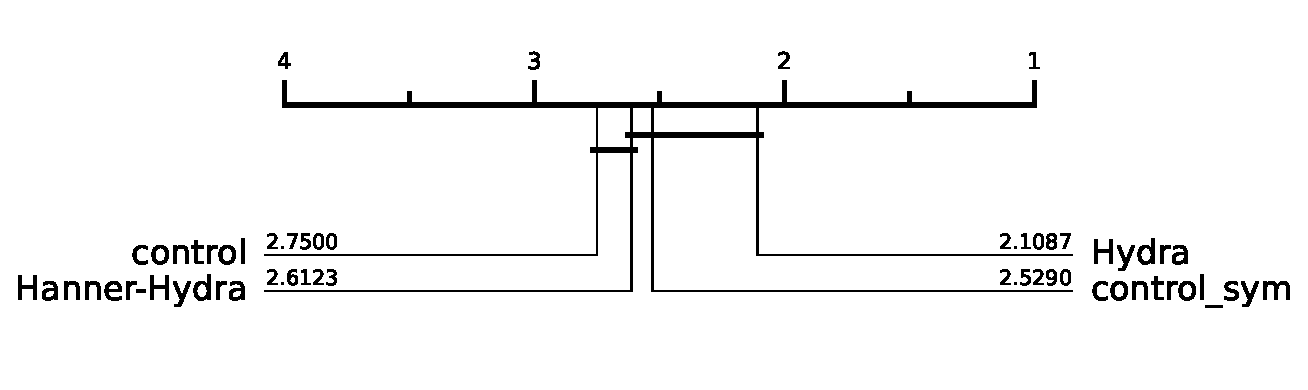
\includegraphics[width=0.8\linewidth]{figures/cd_all}
\caption{Critical-difference diagram over all 138 datasets: average ranks, with cliques
drawn by aeon's convention (one-sided Wilcoxon tests at a fixed level $\alpha/(k-1)$). The
pre-registered frequentist test is the Holm procedure of Table~\ref{tab:wilcoxon}; the
diagram can split pairs that the table does not.}
\label{fig:cd}
\end{figure}

The frequentist analysis agrees (Table~\ref{tab:wilcoxon}). No pair of arms differs
significantly at $\alpha=0.05$ after Holm's correction. A Friedman test over the four arms
is significant ($p=0.0002$), because Hydra ranks first more often: the average ranks are
2.11 for Hydra, 2.53 for \texttt{control\_sym}, 2.61 for \hh{} and 2.75 for
\texttt{control} (Figure~\ref{fig:cd}). On the subsets, two pairs reach significance:
\texttt{control\_sym} against Hydra on UEA ($-0.77$ points, Holm-adjusted $p=0.017$), and
\texttt{control\_sym} against \texttt{control} on UCR ($+0.09$ points, $p=0.045$), a
negligible effect of central symmetry.

\subsection{Comparison with published results}

\begin{table}[t]
\centering\small
% Generated by experiments/paper_tables.py; do not edit by hand.
\begin{tabular}{lrrlcl}
\toprule
Hanner-Hydra vs & Means (\%) & $\Delta$ & W/T/L & $P$(left / rope / right) & Label \\
\midrule
WEASEL 2.0 & 87.40 vs 87.38 & $+0.01$ & 58/3/51 & 0.441 / 0.080 / 0.479 & inconclusive \\
MiniRocket & 87.40 vs 87.44 & $-0.05$ & 57/4/51 & 0.474 / 0.110 / 0.416 & inconclusive \\
MultiRocket & 87.40 vs 88.14 & $-0.75$ & 42/5/65 & 0.991 / 0.003 / 0.007 & practically worse \\
HIVE-COTE 2.0 & 87.40 vs 89.14 & $-1.75$ & 30/4/78 & 1.000 / 0.000 / 0.000 & practically worse \\
\bottomrule
\end{tabular}

\caption{\hh{} against aeon's published 30-resample results on the 112 UCR datasets
(dataset means). Bayesian signed-rank test, ROPE $\pm0.5$; \emph{practically worse}:
$P(\Delta<-0.5)\ge0.95$.}
\label{tab:published}
\end{table}

Table~\ref{tab:published} compares \hh{} with the published results of four other methods
on the UCR datasets; aeon publishes these results for UCR only. \hh{} is on par with
WEASEL~2.0 and MiniRocket: the mean differences are below 0.05 points, but the posterior
is split between the two sides of the ROPE, so neither equivalence nor a difference is
shown. It is practically worse than MultiRocket ($-0.75$ points) and HIVE-COTE~2.0
($-1.75$). In two-sided Wilcoxon tests over all pairs of the eight methods (our four arms
and the four published ones), only HIVE-COTE~2.0 differs significantly from \hh{} ($p=2\times
10^{-6}$, $5\times10^{-5}$ after Holm's correction over 28 pairs). The published results use
different resample splits from ours, so this comparison is paired by dataset, not by
resample; our Hydra arm agrees with aeon's published Hydra results ($+0.33$ points,
posterior entirely in the ROPE).

\subsection{Ablations}

\begin{table}[t]
\centering\small
% Generated by experiments/paper_tables.py; do not edit by hand.
\begin{tabular}{lrrrlrr}
\toprule
Variant & Datasets & Mean (\%) & $\Delta$ vs default & W/T/L & $P$(rope) & $\Delta$ vs Hydra \\
\midrule
\texttt{center=False} & 138 & 83.69 & $-0.68$ & 26/8/104 & 0.995 & $-0.74$ \\
\texttt{center=True} & 138 & 84.35 & $-0.02$ & 60/8/70 & 1.000 & $-0.08$ \\
\texttt{features=hydra} & 138 & 84.37 & $+0.00$ & 0/138/0 & 1.000 & $-0.06$ \\
\texttt{max\_channels=32} & 7 & 65.78 & $-0.90$ & 2/0/5 & 0.285 & $-2.09$ \\
\texttt{max\_channels=auto} & 7 & 66.14 & $-0.53$ & 3/0/4 & 0.550 & $-1.72$ \\
\bottomrule
\end{tabular}

\caption{Exploratory ablations of \hh{}, 30 resamples each. $\Delta$ against the default
configuration (mixed centring, at most 8 channels, soft-max and hard-max counts) and
against Hydra; $P$(rope) from the Bayesian signed-rank test against the default. The
\texttt{max\_channels} variants differ from the default only on the 7 datasets with
$C\ge18$.}
\label{tab:ablations}
\end{table}

Table~\ref{tab:ablations} reports the pre-registered ablations, which are exploratory.
Without centring, accuracy drops by 0.68 points on average, mostly on UCR, and \hh{} loses
104 of the 138 datasets to the default. Most losses are small, though: the median is 0.24
points, 62\% of the datasets change by at most 0.5 points, and one dataset,
PigAirwayPressure, loses 27.9 points and alone moves the mean from $-0.49$ to $-0.68$. The
signed-rank test is robust to such an outlier, so its posterior lies in the ROPE
($P=0.995$). Centring every group instead of every second one is
equivalent to the default. Hard-min counts in place of the hard-max counts give the same
accuracy on all 4,140 dataset resamples, and all 4,140 prediction files are
byte-identical to those of the default. This confirms the permutation argument of Proposition~\ref{prop:hardmin}
in the implementation, which takes the minimiser as the antipode of the maximiser; it is not
a test of Hydra's first-minimiser rule. Larger channel subsets do not help on the 7 high-channel datasets ($-0.90$ and $-0.53$
points; W/T/L 2/0/5 and 3/0/4, $P(\text{rope})=0.285$ and $0.550$, so inconclusive), which
makes a lack of channel coverage an unlikely explanation for the UEA gap.
